\documentclass{rbfin}
\usepackage{amsmath}
\usepackage{amssymb} %mathbb
\usepackage{gensymb} % \degree
\usepackage{graphicx}
\usepackage{hyperref}
\usepackage{cancel}
\newcolumntype{C}{>{$}c<{$}}


\begin{document}
\selectlanguage{brazil}
\shorttitle{Identificação de Sistemas e Estimação de Parâmetros 2022} % appears on header every other page
\rbfe{}
\autor{Vinícius Claudino Ferraz, 2022}


\large

\begin{center}
LISTA 2
\end{center}

\normalsize

\doublespacing

\section*{Questão 1}

O ruído branco é nu:

\begin{center}
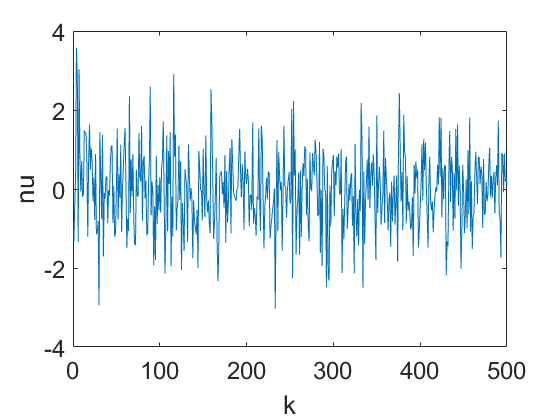
\includegraphics[scale=0.666]{1nu}
\end{center}

Combinado com o ruído branco, geramos a entrada u:

\begin{center}
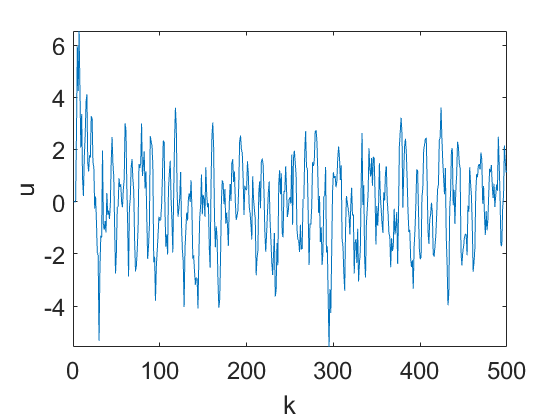
\includegraphics[scale=0.666]{1u}
\end{center}

\newpage

A autocorrelação da entrada é:

\begin{center}
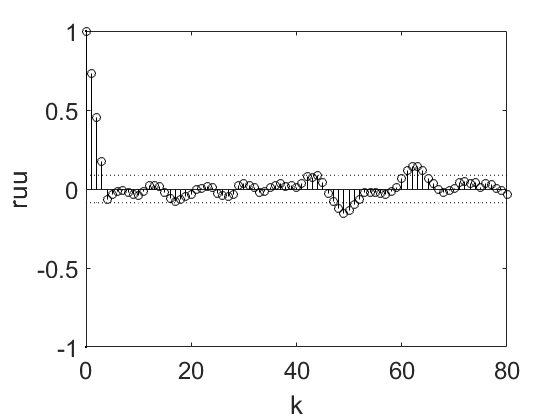
\includegraphics[scale=0.666]{1ruu}
\end{center}

Repare que basicamente ela só fica maior que a faixa de confiança de $0$ a $3$, como exige a fórmula. Isso também ocorre na correlação entre u e nu. A partir de $k = 44$, os cálculos não permitem falar em confiança seguramente.

Veremos agora que o ruído não é autocorrelacionado. A autocorrelação do ruído é:

\begin{center}
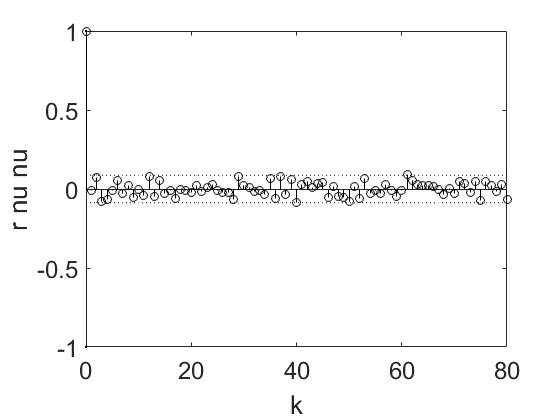
\includegraphics[scale=0.666]{1rnunu}
\end{center}

\newpage

A correlação entre u e nu é:

\begin{center}
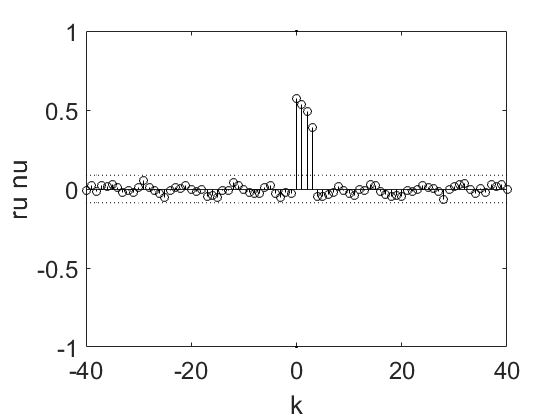
\includegraphics[scale=0.666]{1runu}
\end{center}

\section*{Questão 2}

a) A simulação de $H(z)$ gerou os gráficos:

\begin{center}
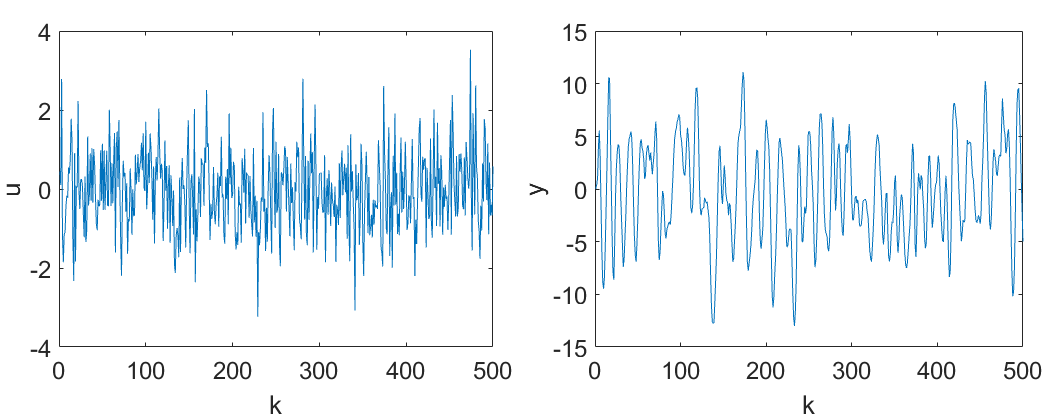
\includegraphics[scale=0.65]{2a}
\end{center}

\newpage

b) As correlações desejadas são:

\begin{center}
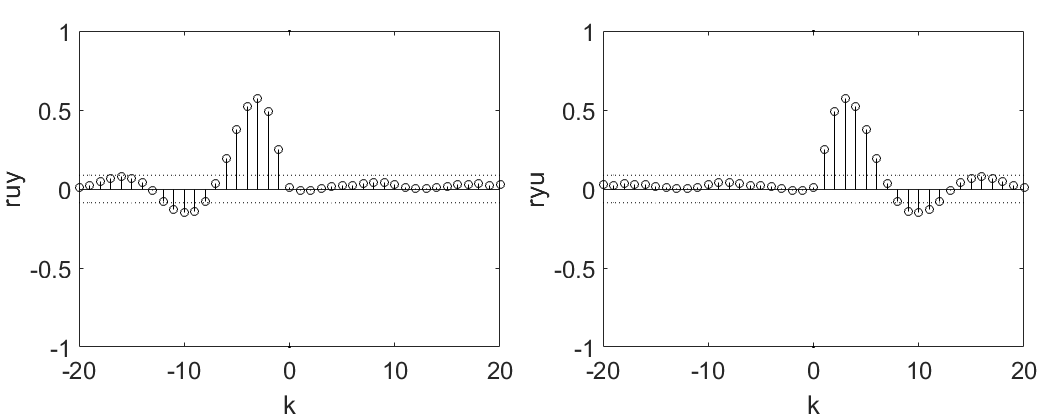
\includegraphics[scale=0.65]{2b}
\end{center}

Repare que existe correlação apenas nos $k$ iniciais.

c) A estrutura da função myccf retorna valores positivos $(r > 0)$ à direita $(k > 0)$ quando a saída é a primeira coluna e a entrada é a segunda coluna do parâmetro.

d) Os gráficos abaixo mostram que a coluna $1$ do arquivo de dados faz papel de entrada $u$, assim como a coluna $2$ faz papel de saída $y$. A correlação é grande, não sabemos se vai diminuir quando $k \to +\infty$.

\begin{center}
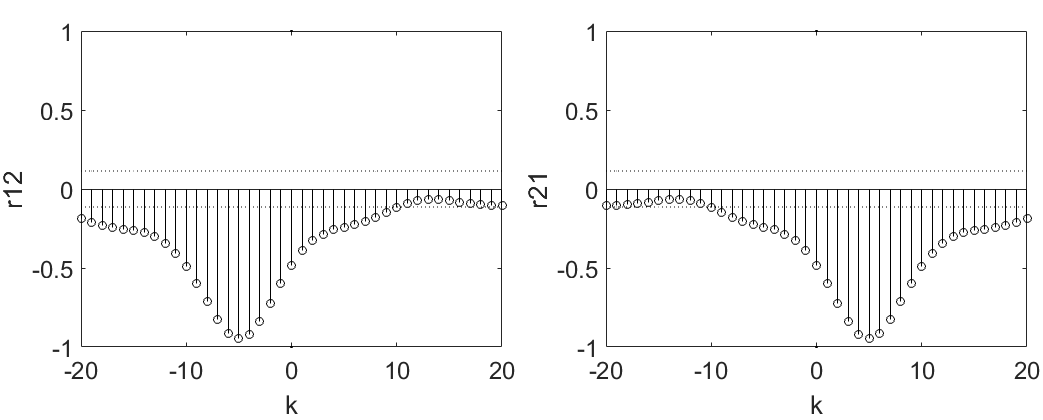
\includegraphics[scale=0.65]{2d}
\end{center}

\newpage

\section*{Questão 3}

Utilizei como entrada $u = prbs(500,6,1)$. A saída somada com o ruído é:

\begin{center}
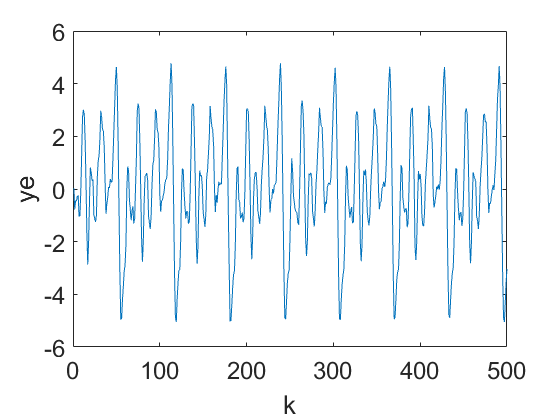
\includegraphics[scale=0.666]{3ye}
\end{center}

As correlações utilizadas na equação de Wiener-Hopf são:

\begin{center}
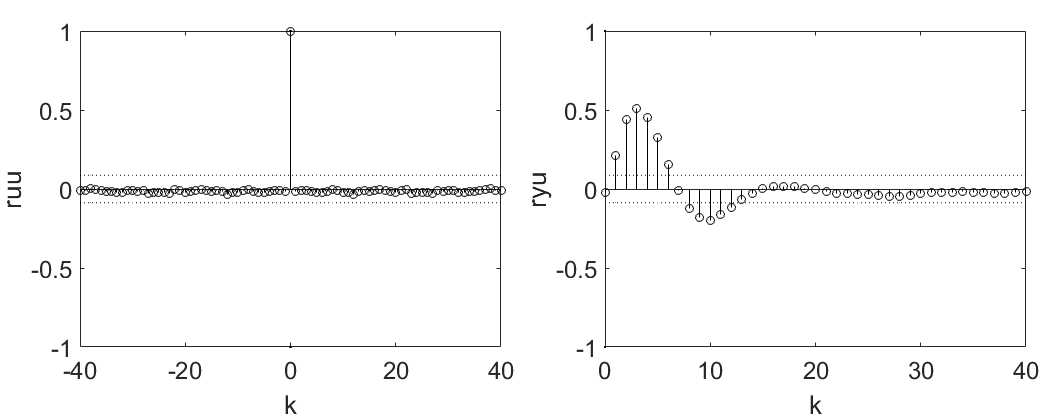
\includegraphics[scale=0.65]{3r}
\end{center}

\newpage

Plotamos a resposta ao impulso ideal seguida da estimada e obtivemos:

\begin{center}
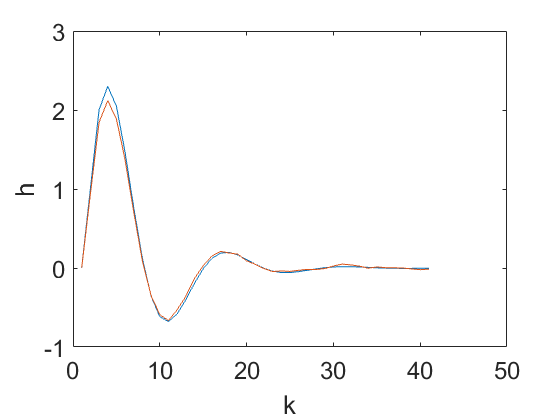
\includegraphics[scale=0.666]{3h}
\end{center}

\section*{Questão 4.19}

O arquivo prsba02.dat tem três colunas: $t,u,y$. Verificando, obtivemos:

\begin{center}
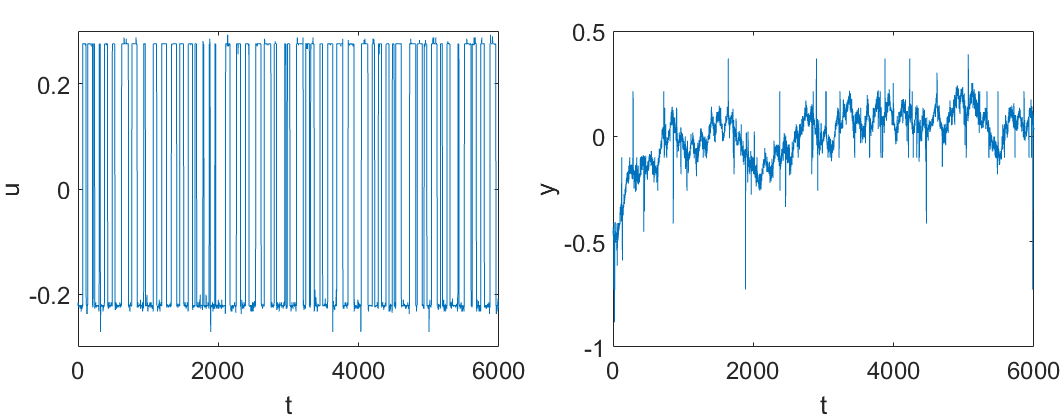
\includegraphics[scale=0.65]{4uy}
\end{center}

\newpage

Repetimos o procedimento da questão $3$. As correlações utilizadas na equação de Wiener-Hopf são:

\begin{center}
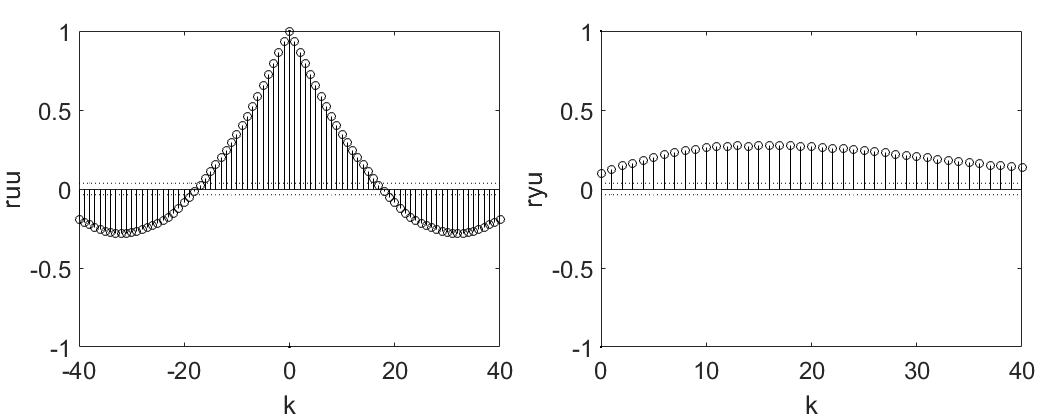
\includegraphics[scale=0.65]{4ruu}
\end{center}

Plotamos a resposta ao impulso estimada versus a primeira coluna $(t)$ e obtivemos:

\begin{center}
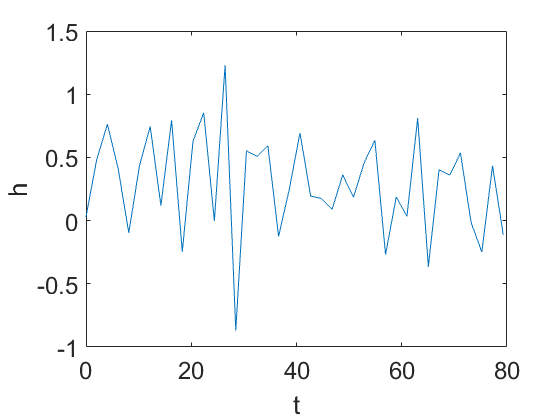
\includegraphics[scale=0.666]{4h}
\end{center}

\section*{Questão 4.20}

O sistema, com condições iniciais nulas, é: $\cfrac{Y(s)}{U(s)} = \cfrac{1}{1000s + 1} = 0.001 \cfrac{1}{s + 0.001}$

Pelo Laplace inverso, $h(t) = 0.001 \exp(- 0.001\,t)$; $t \ge 0$.

$1000 s Y(s) + Y(s) = U(s) \Rightarrow 1000 y'(t) + y(t) = u(t) \Rightarrow y'(t) = \cfrac{u(t) - y(t)}{1000}$. 

\newpage

Plotamos a resposta ao impulso, via simulação:

\begin{center}
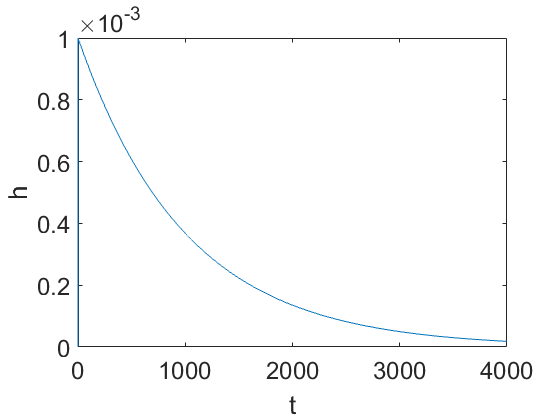
\includegraphics[scale=0.666]{5h}
\end{center}

Para $T_b = 1$, obtivemos:

\begin{center}
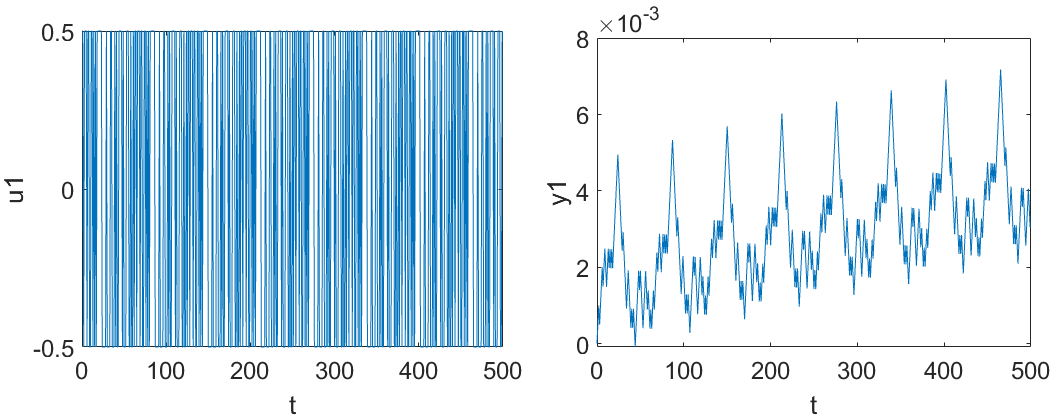
\includegraphics[scale=0.65]{5u1}
\end{center}

\newpage

Para $T_b = 100$, obtivemos:

\begin{center}
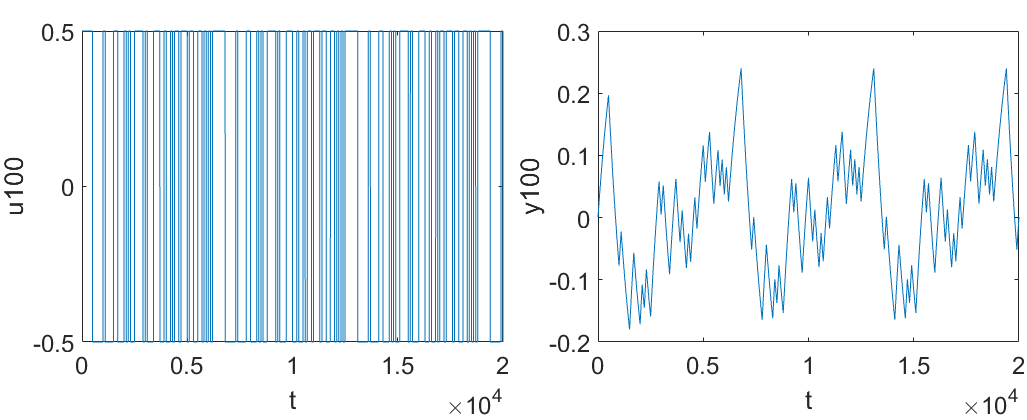
\includegraphics[scale=0.65]{5u100}
\end{center}

Para $T_b = 1000$, obtivemos:

\begin{center}
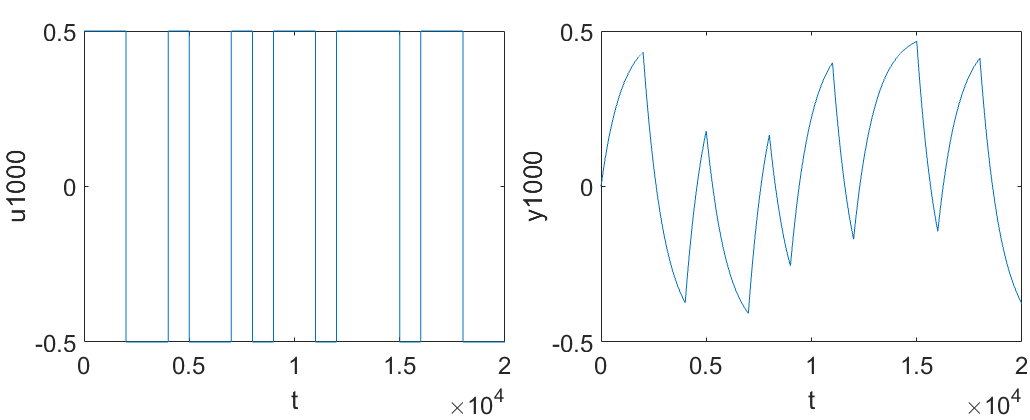
\includegraphics[scale=0.65]{5u1k}
\end{center}

\newpage

Para $T_b = 10000$, obtivemos:

\begin{center}
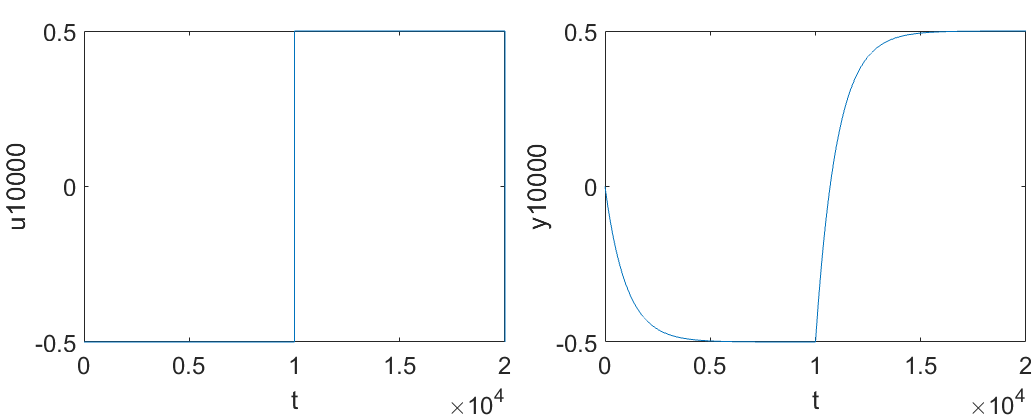
\includegraphics[scale=0.65]{5u10k}
\end{center}

Aparentemente, para $T_b > 100$, a taxa de oscilação não é mais suficiente para garantir aleatoriedade, e o sinal de entrada não é mais adequado para identificação via correlações.

\vspace{6mm}

Link para os \href{https://drive.google.com/file/d/15xBpWf6KBn7H9UEi94khlrKB8rwDWyDS/view?usp=sharing}{\color{blue}\underline{códigos-fonte}}.

Versão de 06/maio/2022\footnote{Fora da caridade não há salvação.} por Vinicius Claudino Ferraz. 

Matrícula: 2019435823.

\end{document}
